
\newpage

\begin{tikzpicture}[remember picture,overlay]
  \node[anchor=north west,outer sep=0,inner sep=0] (img) at (current page.north west) {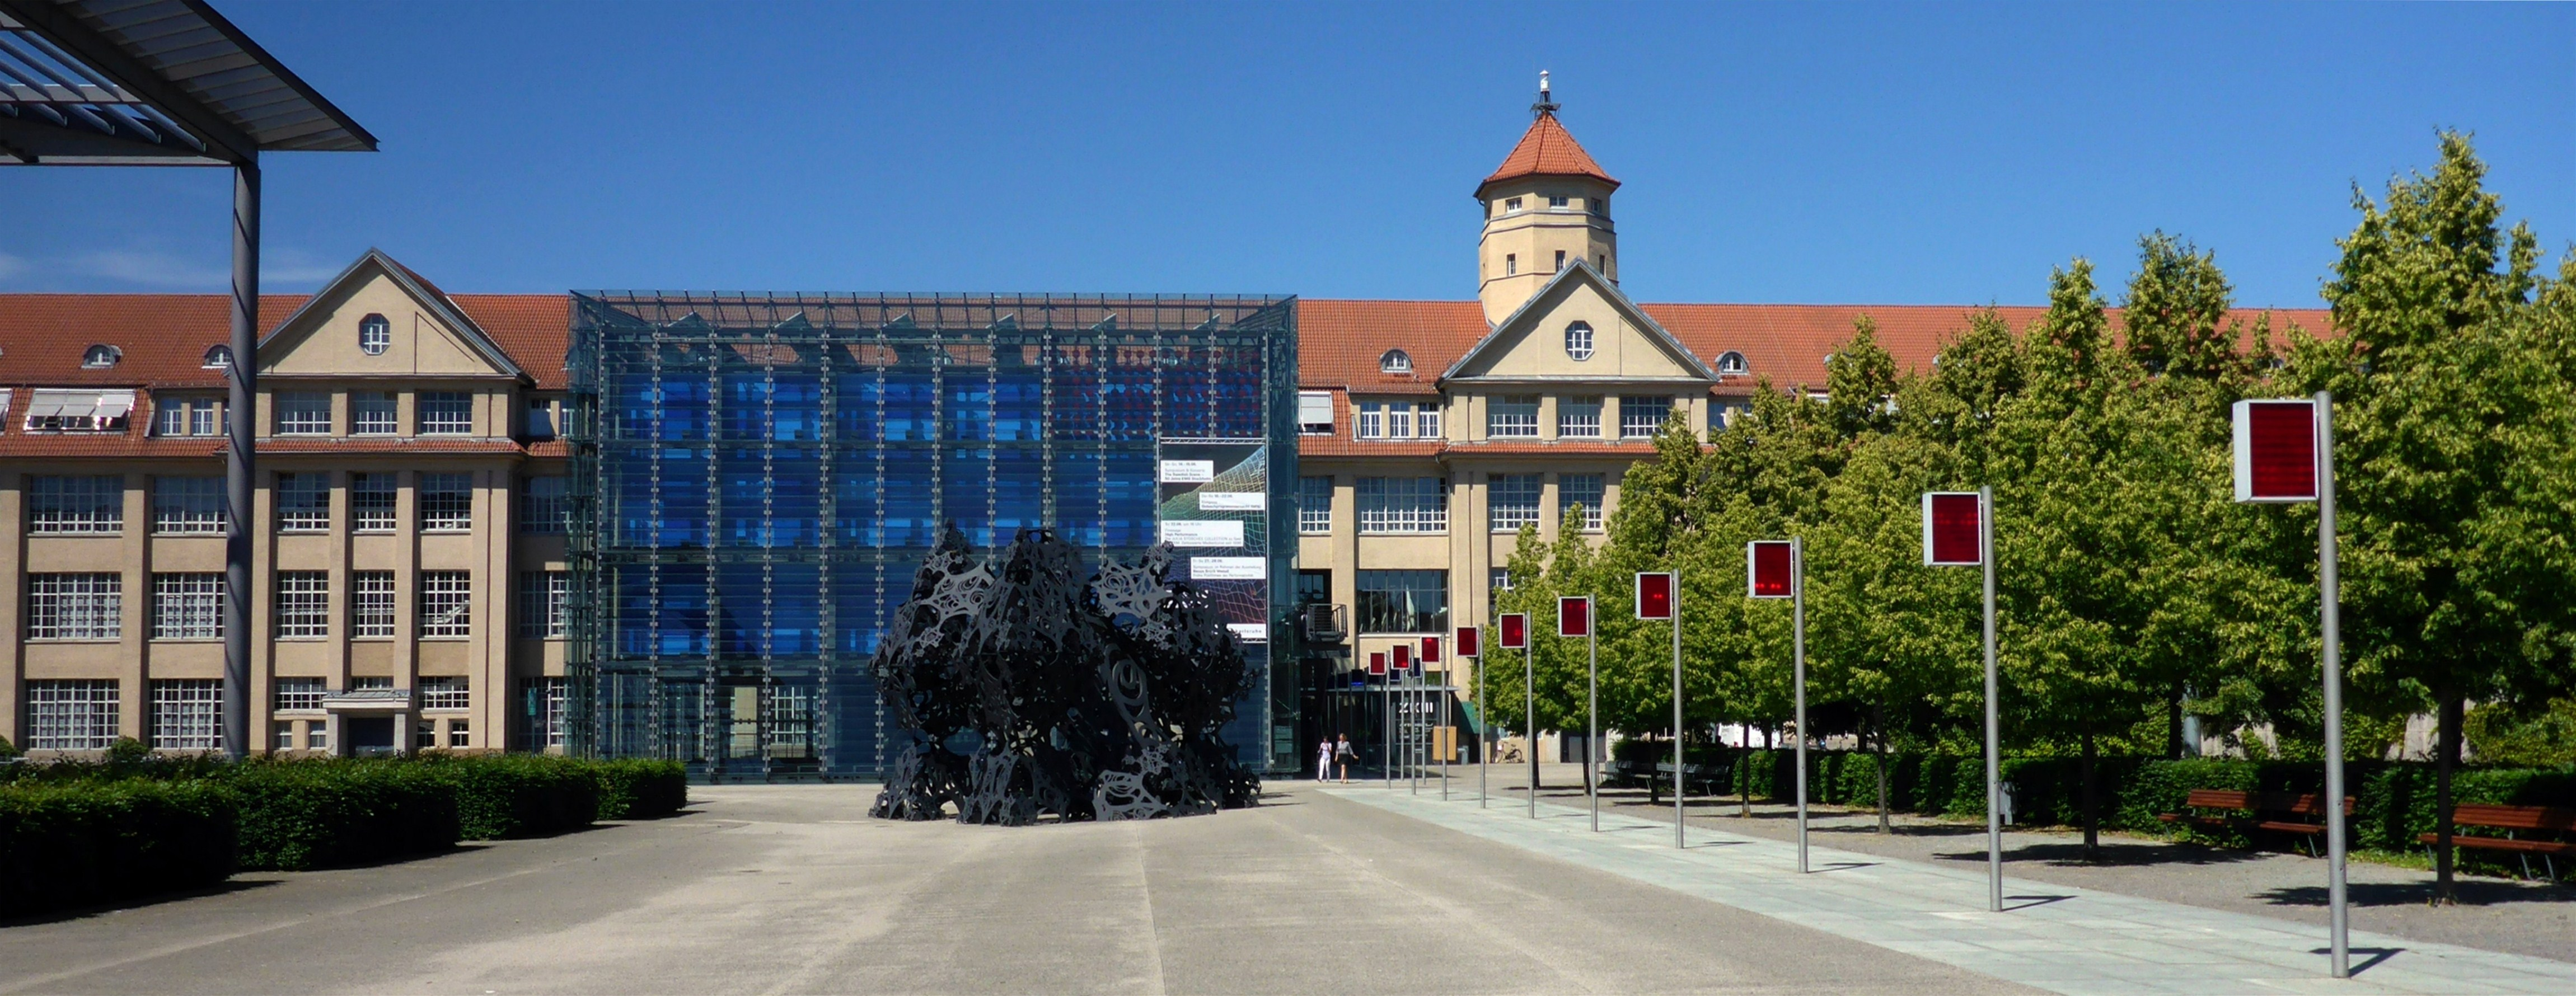
\includegraphics[width=21cm]{images/city/zkm-2.jpg}};
  \node[anchor=south west,outer sep=1ex,color=white] at (img.south west) {\imgtitle{Günter Josef Radig}{ZKM}{CC BY-NC-SA 2.0, not modified, \url{http://ka.stadtwiki.net/Datei:ZKM_2014.JPG}}};
\end{tikzpicture}

\vspace*{5cm}

\section{Travel}

Karlsruhe is a generally well connected city. While it does not have a major
international airport of its own, there are numerous airports well within reach
to allow both overseas and european visitors a cost effective journey. The city
is well connected to the Deutsche Bahn ICE/IC train network and also offers
direct TGV connections to Paris and Marseille (via Lyon). In addition to this
there are numerous far distant bus routes connecting Karlsruhe with destinations
all over Europe.

\begin{multicols}{2}
\raggedcolumns

\subsection{Frankfurt Airport (FRA)}

Frankfurt Airport (FRA) is germanies busiest airport and an important hub for
international air travel.
\begin{tabbing}
\hspace*{2.5cm} \= \kill
Distance: \> 130\,km \\
By Train: \> 1\,h, $\SI{40}{\euro}$ \\
By Bus:   \> \SI{1.5}{h}–\SI{4}{h}, $\ge\SI{10}{\euro}$
\end{tabbing}

\subsection{Stuttgart Airport (STX)}

About 55 airlines are flying to over a 100 destinations from Stuttgart airport.
It is reachable both by S-Bahn and train or using far distance busses.

\begin{tabbing}
\hspace*{2.5cm} \= \kill
Distance: \> 80\,km \\
By Train: \> \SI{1.5}{\hour}, $\SI{28}{\euro}$ \\
By Bus:   \> \SI{1}{\hour}, $\ge\SI{5}{\euro}$
\end{tabbing}

\subsection{Karlsruhe Baden (FKB)}

Karlsruhe Baden Airpark is a small airport located to the south of the city. It
mostly hosts cheaper airline companies flying to holiday destinations
throughout europe.

\begin{tabbing}
\hspace*{2.5cm} \= \kill
Distance: \> 45\,km \\
By Tram/Bus: \> \SI{1}{\hour}, $\SI{7.10}{\euro}$ \\
\end{tabbing}

\subsection{Strasbourg/Entzheim (SXB)}

This airport located just south of Strasbourg can easily be reached from Karlsruhe
using local trains.

\begin{tabbing}
\hspace*{2.5cm} \= \kill
Distance: \> 105\,km \\
By Tram/Bus: \> \SI{2}{\hour}, 20 to $\SI{30}{\euro}$ \\
\end{tabbing}

\end{multicols}

